\section{Jonathan}
\subsection{Overview}
\begin{frame}{Jonathan: Overview}
\begin{itemize}
\item Collaborations
\item New Stuff
\end{itemize}
\end{frame}

\subsection{GUI Requirements Analysis}
\begin{frame}{GUI Requirements Analysis}
A collaboration between SW609, SW610 and SW612.\\

A couple of the more noteworthy questions from the first meeting:
\begin{itemize}
\item How should switching from Guardian to Citizen and back happen?
\item Can there be multiple Guardians pr. Citizen?
\item Who are supposed to login?
\end{itemize}

\end{frame}

\begin{frame}[fragile]{GUI Requirements Analysis}
A couple of the more noteworthy requirements:

\begin{itemize}
\item There needs to be an option for grayscale.
\item If the system crashes it needs to return to a stable state or return to the Launcher
\item The QR-system needs to be replaced by a password based system.
\item Citizens should not be logged out automatically.
\item There should be an institute type user.
\end{itemize}

Based on the requirements for the users we created this diagram:
\includegraphics[scale=0.5]{figures/LoginDiagram.PNG}
\end{frame}

\subsection{REST Architectural Design}
\begin{frame}{REST Architectural Design}
A Collaboration between SW609, SW610, SW613 and SW615.\\

\textbf{skal nok rettes lidt til}
The old client/server has serious problems, therefore make a new using the REpresentational State Transfer (REST) model which has the following requirements:
\begin{itemize}
\item Client-Server: Seperate the user interface from data storage and manipulation.
\item Stateless: Each request to the server returns a response which contains all information required for the client to service the request.
\item Cacheable: Responses from the server must implicitly or explicitly declare themselves as either cacheable or not, in order to prevent the client from reusing expired data.
\item Layered System: The client is incapable of determining if it is connected to the main server or an affiliated intermediate entry point.
\item Uniform Interface: The retrieved data is conceptually different from the representation used on the server. Given a set of data, the client should have enough information to edit and delete the respective information of the server.
\end{itemize}
\end{frame}

\begin{frame}{REST Architectural Design}
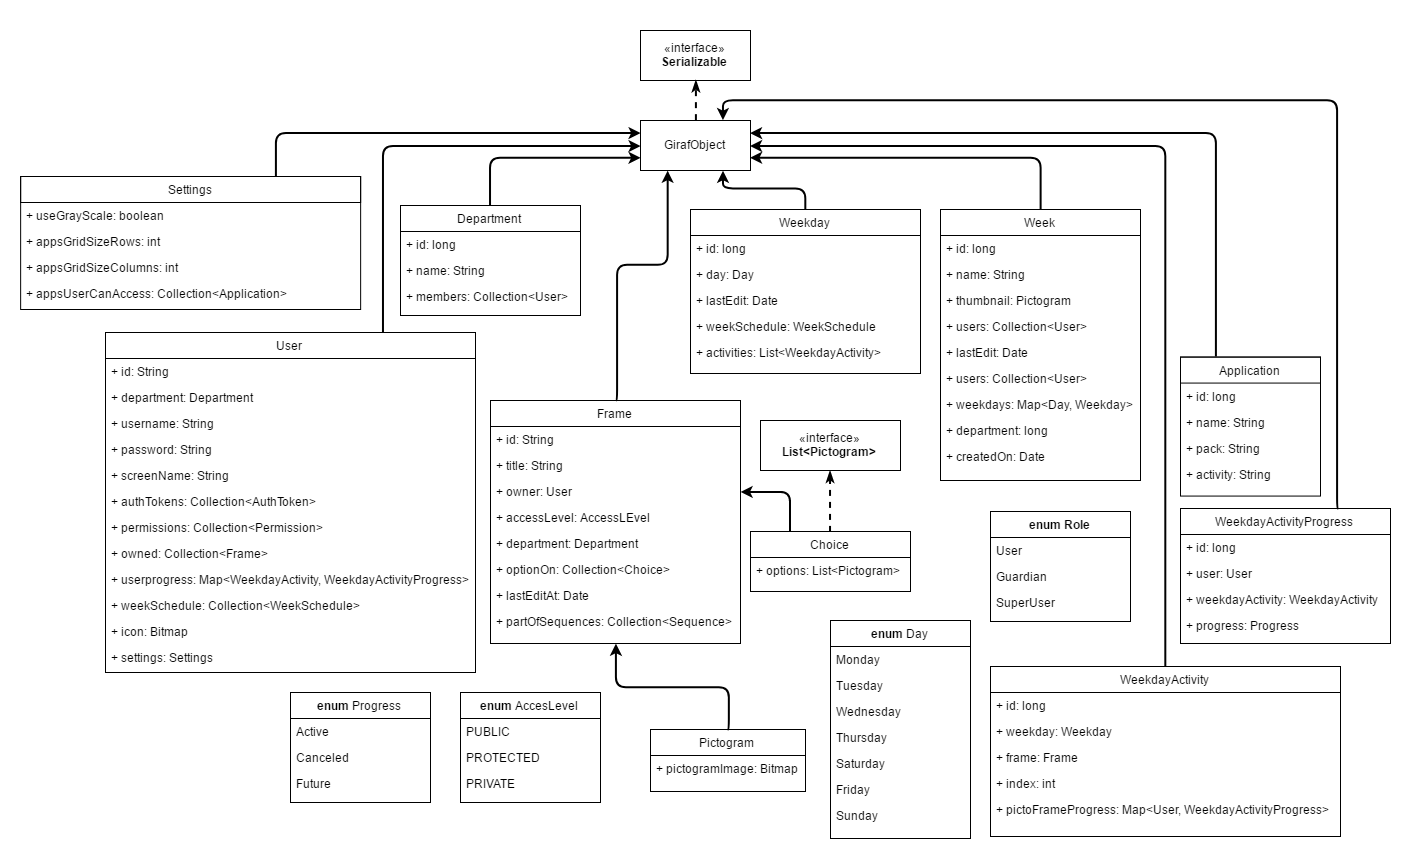
\includegraphics[scale=0.5]{figures/Giraf_RestModelV3.PNG}
\end{frame}

\begin{frame}{REST Architectural Design}

\textbf{WIP}
We use 3 different types of requests:
\begin{itemize}
\item LoginRequest
\item GetRequest
\item PutRequest
\end{itemize}

We also implement VOLLEY which means it is not easy to requests neat.

What is a Request and how do we use it? (hint: RequestQueue and Handler)
\end{frame}

\begin{frame}{REST Architectural Design}
Add a couple of example requests.
\end{frame}

% \subsection{Network Structure}
% \begin{frame}{Network Structure}
% \begin{itemize}
% \item What does the network look like?
% \item Which features are used and how are their domains defined?
% \end{itemize}
% \begin{figure}
%   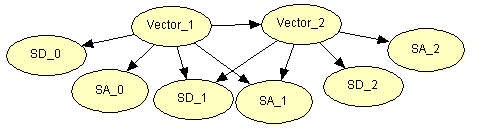
\includegraphics[scale=0.8]{figures/BNDone.PNG}
% \end{figure}
% \end{frame}
